%
%
%
\documentclass[11pt,letterpaper]{article}
\usepackage{naaclhlt2013}
\usepackage{times}
\usepackage{latexsym}
\usepackage{graphicx}
\usepackage{tabularx}
\setlength\titlebox{6.5cm}    % Expanding the titlebox

\title{SemEval 2015 Task 1: Paraphrase and Semantic Similarity in Twitter}
\author{
	Michael Meding\\
  	University Massachusetts Lowell\\
	1 University Ave\\
	Lowell, MA 01854, USA\\
   {\tt mikeymeding@gmail.com}
	\And  
   Hoanh Nguyen\\
	University Massachusetts Lowell\\
	1 University Ave\\
	Lowell, MA 01854, USA\\
	{\tt hoanh.lam.nguyen@gmail.com }
}
\date{}
%	PAPER MUST INCLUDE
% a. an abstract, describing briefly what you have done and results you obtained
%   b. an introduction, a statement of the problem you are trying to address and a brief description of your solution
%   c. related work section, describing relevant results from other people's efforts to solve this problem
%   d. description of your methodology, including 
%       - machine learning methods, 
%       - data sets used in the study,
%       - experimental setup and and evaluation methods;
%   f. description of your results.
%   g. discussion of results, conclusions of your study, future directions for this work
\begin{document}
\maketitle

\begin{abstract}
This paper details the methods and approach we used in an attempt to improve the baseline results of the paraphrase and semantic similarity in Twitter task for the 2015 SemEval competition. The participants are given two sentences and are asked to determine whether the sentences express either the same or a very similar meaning. Then the participants have the option to assign a degree score between 0 and 1. Based on the literature on paraphrase identification, we evaluated system performance primarily by the F-1 score and accuracy against human judgements. 
\end{abstract}

\section{Introduction}
\paragraph{} 
Semantic Evaluation, or SemEval, is an ongoing series of evaluations of computational semantic analysis systems; it evolved from the Senseval word sense evaluation series. The evaluations are intended to explore the nature of meaning in language. We chose SemEval task 1 from the 2015 SemEval series for this project which involves paraphrase and semantic similarity in Twitter. Participants of this task are given two sentences and are asked to determine whether the sentences express either the same or a very similar meaning. Then the participants have the option to assign a degree score between 0 and 1. Based on the literature on paraphrase identification, we evaluated system performance primarily by the F-1 score and accuracy against human judgements. 
\paragraph{}
Our first task with this project was to translate the original starting code from Python to Java. This required rewriting both the main logistic regression function to a Hidden Markov Model that,at this time has no hidden layers. A portion of our rewriting was dedicated to the representation of the data, which we both agreed was poor in the python model. This required us to rewrite the data parser, so it would interface with the same data but in a manner that would also interact nicely with our Java based Hidden Markov Model. Doing this required a significantly longer amount of time than we had initially intended. We also researched further topics and ideas for features for when this implementation was finished. When this Python to Java conversion was finally finished and receiving F-Scores nearly equal to those of the original python code, we began experimenting with several features that we were both familiar with. Such as SentiWordNet because this lexical resource was pivotal in our prior project.

\section{Baseline}
\paragraph{}
The baseline implementation used a logistic regression model and simple lexical features. These features made use of unigrams, bigrams, and trigrams of both the words and the porter stem of the words. It is calculated by the precision, recall, and the F1 Score. The precision is the intersection verses original ngrams. Recall is the intersection verses candidate ngrams. The F1 Score, or F-Score, is a measure of both precision and accuracy combined. Improving the F-Score was our primary objective for this project. Our reimplementation of the baseline was able to achieve an F1 score of just over 0.50 on the development set after training on the supplied training set. This was only slightly worse than the Python logistic regression model that was provided. The results from the given Python baseline was 0.5 for the F-Score, which after some interesting modifications improved to 0.54. The main baseline modification we made focused on excluding the trending topic from the tweet and it put our F-Score right around the starting F-Score of the original Python implementation.

\section{Related Work}
\paragraph{}
In 2014, a similar task appeared in the SemEval competition. It had different data and a slightly different baseline. One of the starting points of our project was to read some of the papers published after this first competition such as \cite{Divergent-Paraphrases} which detailed some of the major teams high level implementations. This allowed us to get a good idea of the approach others had taken. We also saw how some took far more complicated approaches than others. Often the teams which had a well refined and simple supervised approach would do better than those who had chosen to do a complicated unsupervised approach. For example, one group used a simple logistic regression model with several good features and did well in the competition scoring in the top 20. A few groups used a full unsupervised model with co-reference and did not improve on the original baseline.

%Talk about last years twitter project and the related tools that we used from that project

\section{Data}
\paragraph{}
SemEval provided all of its tasks with data to be used for evaluating the results of your work. In our prior Twitter project, we hand annotated our own data set which was extremely time consuming and frustrating. We also did not have any kind of verification of our data set so the accuracy left much to be desired. Luckily, the data sets which were provided to us for this task are both consistent and verified by multiple passes from turkers.
\paragraph{}
The data which was provided consisted of two files, a training data set and a development data set. The training data set consisted of 13063 Tweet pairs and the development data set consisted of 4727 Tweet pairs. These data sets were organized as tab separated values organized as shown by Table~\ref{provided-data}.

%%% SemEval 2015 corpus example table %%%
% | Topic_Id | Topic_Name | Sent_1 | Sent_2 | Label | Sent_1_tag | Sent_2_tag |
%4	1st QB	EJ Manuel the 1st QB to go in this draft	But my bro from the 757 EJ Manuel is the 1st QB gone	(5, 0)	EJ/B-person/NNP/B-NP/O Manuel/I-person/NNP/B-VP/O the/O/DT/B-NP/O 1st/O/CD/I-NP/O QB/O/NNP/I-NP/O to/O/TO/B-VP/O go/O/VB/I-VP/B-EVENT in/O/IN/B-PP/I-EVENT this/O/DT/B-NP/O draft/O/NN/I-NP/O	But/O/CC/O/O my/O/PRP$/B-NP/O bro/O/NN/I-NP/O from/O/IN/B-PP/O the/O/DT/B-NP/O 757/O/CD/I-NP/O EJ/B-person/NNP/I-NP/O Manuel/I-person/NNP/I-NP/O is/O/VBZ/B-VP/O the/O/DT/B-NP/O 1st/O/CD/I-NP/O QB/O/NNP/I-NP/O gone/O/NN/I-NP/O
\begin{table}
\begin{center}
\begin{tabularx}{190pt}{|c|c|}
\hline
\bf Topic ID \\
\hline
\ 4 \\
\hline
\bf Trending Topic Name \\
\hline
\ 1st QB\\
\hline
\bf Sent 1 \\
\hline
\ EJ Manuel the 1st QB to go in this draft \\
\hline
\bf Sent 2 \\
\hline
\ But my bro from the 757 EJ Manuel is\\ 
\ the 1st QB gone \\
\hline
\bf Label \\
\hline
\ (5, 0) \\
\hline
\bf Sent 1 Tagged \\
\hline
\ EJ/B-person/NNP/B-NP/O \\
\ Manuel/I-person/NNP/B-VP/O \\
\ the/O/DT/B-NP/O 1st/O/CD/I-NP/O \\
\ QB/O/NNP/I-NP/O to/O/TO/B-VP/O \\
\ go/O/VB/I-VP/B-EVENT \\
\ in/O/IN/B-PP/I-EVENT \\ 
\ this/O/DT/B-NP/O \\ 
\ draft/O/NN/I-NP/O \\
\hline
\bf Sent 2 Tagged \\
\hline
\ But/O/CC/O/O my/O/PRP\$/B-NP/O \\
\ bro/O/NN/I-NP/O \\ 
\ from/O/IN/B-PP/O the/O/DT/B-NP/O \\
\ 757/O/CD/I-NP/O \\
\ EJ/B-person/NNP/I-NP/O \\
\ Manuel/I-person/NNP/I-NP/O \\
\ is/O/VBZ/B-VP/O the/O/DT/B-NP/O \\ 
\ 1st/O/CD/I-NP/O QB/O/NNP/I-NP/O \\
\ gone/O/NN/I-NP/O \\
\hline
\end{tabularx}
\end{center}
\caption{\label{provided-data} Raw data entry example from the SemEval 2015 Training data set }
\end{table}

\paragraph{}
The "Trending Topic Name" are the names of trends provided by Twitter, which are not hashtags but rather a trending topic between two Tweets, if any exists. This does necessary indicate that a paraphrase exists, only that there is a similar topic between the two. The "Trending Topic Name" from Table~\ref{provided-data} is the text that we removed from both tweets to improve our baseline from .50 to .54.

The "Sent 1" and "Sent 2" are the two sentences, which are not necessarily full tweets. Tweets were tokenized and split into sentences or as close to sentences as Tweets can get.

The "Label" column is in a format such like "(1, 4)", which means among a total of 5 votes 
from Amazon Mechanical turkers only 1 is positive and 4 are negative. We mapped these values to binary labels as follows,
paraphrases: (3, 2) (4, 1) (5, 0), non-paraphrases: (1, 4) (0, 5), ignored: (2, 3) as we are training binary classifier.

The "Sent 1 Tagged" and "Sent 2 Taggged" are the two sentences with part-of-speech and named entity tagging applied. 

\section{Initial Base Line Modification}
\paragraph{}
Our first thought was to see what we could do to improve the baseline. After some time and research, we decided to see what would happen if we simply omitted the trending topic name from both Tweets being compared. Our intuition behind that was if two Tweets share a trending topic which is directly mentioned in both Tweets, then by removing them would expose the true differences between them. If they were still very close after having removed the trending topics then the likelihood that they are paraphrases of each other would be higher. This turned out to be true and is reflected in our results bringing us from below the initial baseline score to right around the original baseline. Additionally, the latter features would make use of ngrams generated from this both before and after the trending topic was removed from the original Tweet.

\section{Ark Tweet NLP}
\paragraph{}
Ark Tweet NLP is a part-of-speech tagger that was built specifically for Tweets by Carnegie Mellon. In a previous project, we created features that looked at n-grams and the part-of-speech tags. Those features worked well but for that project, so we continued on that trend using a similar approach for our current project. For this task, we followed the idea introduced in the original python baseline and calculated the precision, recall, and F1 scores. The actual F1 score on the dev set was just shy of 0.36 for the original python baseline.

\section{Harvard General Inquirer}
\paragraph{}
The Harvard General Inquirer is a lexical resource that provides a number of categories that a word belongs to. There are 182 categories, however most don't show up very often. For our data set, the Harvard Inquirer categories that we settled on were ones that appeared more than 3000 times in the training set. For features, we took a bag of words approach and used the categories found in the original and candidate tweets. Aside from that, we also calculated the precision, recall, and F1 of the mutual category count verses the category count for the original and candidate tweets. The F1 score of these features was just under 0.31.

\section{SentiWordNet}
\paragraph{}
SentiWordNet is a lexical resource that provides sentiment scores for words. Each SentiWordNet entry contains five explicit attributes (part-of-speech, id, positive score, negative score, synset terms, and glossary) and an implicit attribute (objective which is 1 - positive score - negative score). 

%%% SentiWordNet corpus example table %%%
\begin{table}
\begin{center}
\begin{tabularx}{183pt}{|c|c|c|c|}
\hline
\bf POS & \bf P & \bf N & \bf Term \\ 
\hline
\ n & 0 & 0.5 & spoiler\#1 \\
\ n & 0.125 & 0.125 & supermodel\#1 \\
\ n & 0.375 & 0.25 & swaggerer\#1 \\
\ n & 0 & 0.5 & affinity\#2 \\
\hline
\end{tabularx}
\end{center}
\caption{\label{sentiword-table} ~SentiWordNet corpus example. Glossary and ID removed due to size restriction. }
\end{table}

\paragraph{}
The intuition behind using sentiment is that if one statement has a positive sentiment and the other has a negative sentiment then the two Tweets being analysed are unlikely to be discussing the same topic. The features we implemented using SentiWordNet were scores divided by entry count, if there are more negative entries than positive entries, scores divided by non-zero score entry count, scores for adjectives divided by non-zero score entry count, and binary features for majority counts. These features looked at each statement individually. Most of these features were inspired by Opinion Mining Using SentiWordNet paper \cite{Paraphrase-Identification}.
Some features that looked at both statements were binary features that check if both had majority score or counts. The F1 score of these features was around 0.06.
\paragraph{}
Our first experiment, after establishing a good baseline, was to score the tweets based on word level sentiment. We preformed a crude run with sentiment weighted heavily to see if we could get any kind of result. This unfortunately was quite bad, and did not yield an improvement of any kind. We pushed a bit further by attempting to score the entire tweet and getting an average for comparison, but the results were equally as bad. During this time we had acquired Willie Boag's Twitter sentiment code, from a prior SemEval competition, to see if his sentiment analyser could improve on our crude model. However, after seeing the dismal results using only a crude model we decided that it would be of more value to pursue other features to improve our model.

\section{MPQA Subjective Lexicon}
\paragraph{}
The MPQA Subjectivity Lexicon contains entries and provide the strength of the subjectivity and polarity. For this resource, we created a number of binary features. The features compare the number of negative polarity counts to positive polarity counts. Another feature was designed to compare the total number of weak counts to strong counts and negative counts to positive counts. The F1 score of these features was about 0.13. 

\section{Wordnet Synonym}
\paragraph{}
WordNet is a large lexical database of English. Nouns, verbs, adjectives, and adverbs are grouped into sets of synonyms called synsets. Synsets are interlinked by of semantic and lexical relations. This is similar to Thesaurus because it groups words together based on their meanings. However, there are some differences. First, WordNet interlinks not just words as strings of letters but also specific senses of words. As a result, words that are found in close proximity to one another in the network are semantically disambiguated. Second, WordNet labels the semantic relations among words, whereas the groupings of words in a thesaurus does not follow any explicit pattern other than meaning similarity \cite{wordnet}.
\paragraph{}
For our implementation of Wordnet, we took all the words, got all the synonyms for all words in a given tweet, and placed all of it in to a set. Then we calculate the precision, recall, and F-Score in a similar way to that of our baseline, except we calculate the intersection from the words to the words and their synonyms in the second given Tweet. The F-Score, after applying this method, close to 0.54 which can be seen in our results Table~\ref{final-results-dev}.

\section{Harvard Inquirer with Wordnet Synonym}
\paragraph{}
Since the WordNet synonym feature worked well we decided to combine it with the Harvard Inquirer feature. We used the Harvard Inquirer features with the all of the words and their synonyms. With more words being put into the Harvard Inquirer feature our chances of a flag being turned on was slightly higher. We also operating under the assumption that synonyms tend to be in the same categories as their root word. While these two features combined had slightly better precision they did not have as good recall. Our final results therefore were quite low, only achieving an F-Score of 0.25 on the development set.

\section{Chat Speak Translator}
\paragraph{}
After spending some time looking at the raw data and attempting to come up with ways to improve our numbers, we noticed that the data contained chat speak abbreviations such as "QB," for quarter-back, or "TTY," for talk to you later, which was common in our data set. So to attempt to normalize this, we used a chat speak translation lexicon built from the Netlingo chat speak dictionary. The lexicon is simple with simply tab separated values with the initialism on one side and the translation on the other.
\paragraph{}
Of course one would expect that by normalizing these values we would see some improvement reflected in our results. Strangely however, normalizing the values actually had the opposite effect. We saw all values, precision, recall, and F-score suffer by around .01 as shown by comparing the results shown in Table~\ref{chatspeak-without-table} and Table~\ref{chatspeak-with-table}.

\section{Final Results}
After trying several neural network configurations incorporating a mix of features, we ended up with something that was slightly better than our modified base features. Simply using all of the features we developed gave us a score which was worse than our best feature alone. Our final configuration was a two layer neural network using the modified base features, Ark Tweet, Harvard General Inquirer, and WordNet synonyms. This gave us a final F-Score of 0.57 as can be seen in the table on Page~\pageref{SemEval2015-Results}.

%\section{Future Improvements}
%blah blah blah blah blah blah blah blah blah blah blah blah blah blah blah blah blah blah blah 


\section*{Acknowledgments}
\paragraph{}
We would like to acknowledge {\bf Alison Rose} for her ability to edit our horrible grammar despite not knowing what we are even writing about. Without her skills this paper would have been near unreadable.

%%%%%%%%%%%%%%%%%%%%%%%%%%%%%%%%%%%%%%%%%%%%%%%%%%%%%%%%%%%%%%%%%%%%%%%%%%%%%%%%%%%%%%%%%%
%%%%%%%%%                     TABLES                                             %%%%%%%%%
%%%%%%%%%%%%%%%%%%%%%%%%%%%%%%%%%%%%%%%%%%%%%%%%%%%%%%%%%%%%%%%%%%%%%%%%%%%%%%%%%%%%%%%%%%


 %%% Without Chatspeak Translator %%%
\begin{table}[p]
\begin{center}
\begin{tabularx}{111pt}{|c|c|}
\hline
\bf Training & \bf Data \\ 
\hline
\ Precision & 0.773 \\
\ Recall & 0.611 \\
\ F1-Score & 0.680 \\
\hline
\bf Development & \bf Data \\ 
\hline
\ Precision & 0.774 \\
\ Recall & 0.416 \\
\ F1-Score & 0.542 \\
\hline
\end{tabularx}
\end{center}
\caption{\label{chatspeak-without-table} Metrics {\bf without} the Chat Speak text preprocessor applied }
\end{table}

 %%% With Chatspeak Translator %%%
\begin{table}[p]
\begin{center}
\begin{tabularx}{111pt}{|c|c|}
\hline
\bf Training & \bf Data \\ 
\hline
\ Precision & 0.762 \\
\ Recall & 0.600 \\
\ F1-Score & 0.672 \\
\hline
\bf Development & \bf Data \\ 
\hline
\ Precision & 0.756 \\
\ Recall & 0.408 \\
\ F1-Score & 0.530 \\
\hline
\end{tabularx}
\end{center}
\caption{\label{chatspeak-with-table} Metrics {\bf with} the Chat Speak text preprocessor applied }
\end{table}

\clearpage

% best, 0.800, 0.760, 0.616, 0.680, 0.757, 0.761, 0.457, 0.571

 %%% Training data set final results %%%
\begin{table}[htp]
\begin{center}
\begin{tabularx}{374pt}{|c|c|c|c|c|}
\hline
\bf feature & \bf train accuracy & \bf train precision &\bf train recall &\bf train F1 \\
\hline
\ \bf best &\bf 0.800 &\bf 0.760 &\bf 0.616 &\bf 0.680 \\
\ base & 0.790 & 0.744 & 0.601 & 0.665 \\
\ mod & 0.792 & 0.763 & 0.578 & 0.658 \\
\ ark & 0.683 & 0.592 & 0.277 & 0.377 \\
\ harvard & 0.688 & 0.614 & 0.266 & 0.371 \\
\ sentiwordnet & 0.674 & 0.661 & 0.121 & 0.205 \\
\ subjective & 0.673 & 0.667 & 0.113 & 0.193 \\
\ wordnet & 0.788 & 0.743 & 0.596 & 0.661 \\
\ harvard \& wordnet & 0.694 & 0.648 & 0.256 & 0.367 \\
\hline
\end{tabularx}
\end{center}
\caption{\label{final-results-train} Our final {\bf training set} results for single layer neural network with softmax }
\end{table}

 %%% Development set data final results %%%
\begin{table}[htp]
\begin{center}
\begin{tabularx}{347pt}{|c|c|c|c|c|}
\hline
\bf feature & \bf dev accuracy &\bf dev precision &\bf dev recall & \bf dev F1 \\
\hline
\ \bf best &\bf 0.757 &\bf 0.761 &\bf 0.457 &\bf 0.571 \\
\ base & 0.735 & 0.746 & 0.384 & 0.507 \\
\ mod & 0.751 & 0.771 & 0.424 & 0.547 \\
\ ark & 0.678 & 0.612 & 0.254 & 0.358 \\
\ harvard & 0.670 & 0.601 & 0.208 & 0.309 \\
\ sentiwordnet & 0.644 & 0.485 & 0.033 & 0.062 \\
\ subjective & 0.646 & 0.509 & 0.074 & 0.129 \\
\ wordnet & 0.745 & 0.748 & 0.422 & 0.540 \\
\ harvard \& wordnet & 0.652 & 0.634 & 0.161 & 0.248 \\
\hline
\end{tabularx}
\end{center}
\caption{\label{final-results-dev} Our final {\bf development set} results for single layer neural network with softmax }
\end{table}

%%% FINAL RESULTS COMPARISION TABLE %%%
%SemEval2015Results.png
\begin{figure*}[htp]
\centering
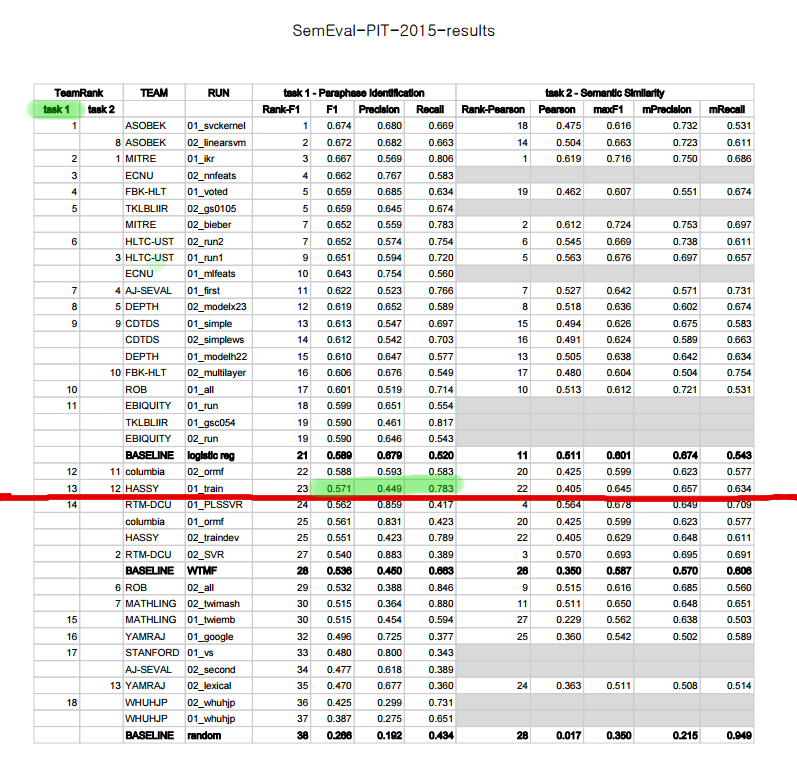
\includegraphics[width=\textwidth, height=\textheight, keepaspectratio]{SemEval2015Results}
\label{SemEval2015-Results}
%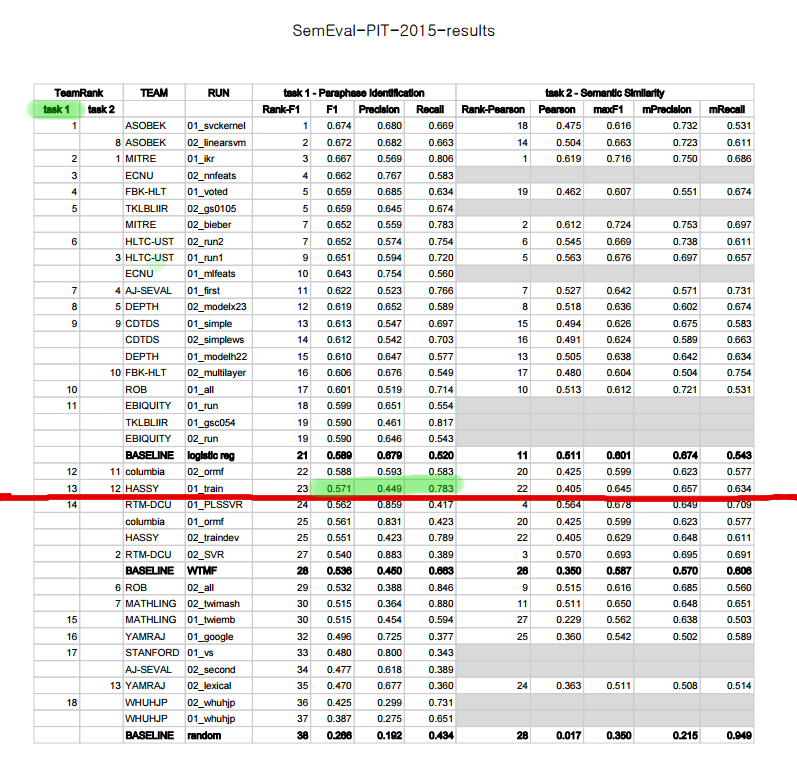
\includegraphics{SemEval2015Results}
\end{figure*}


\clearpage
% features, train_accuracy, train_precision, train_recall, train_f1, dev_accuracy, dev_precision, dev_recall, dev_f1
% base, 0.790, 0.744, 0.601, 0.665, 0.735, 0.746, 0.384, 0.507
% mod, 0.792, 0.763, 0.578, 0.658, 0.751, 0.771, 0.424, 0.547
% ark, 0.683, 0.592, 0.277, 0.377, 0.678, 0.612, 0.254, 0.358
% harvard, 0.688, 0.614, 0.266, 0.371, 0.670, 0.601, 0.208, 0.309
% sentiwordnet, 0.674, 0.661, 0.121, 0.205, 0.644, 0.485, 0.033, 0.062
% subjective, 0.673, 0.667, 0.113, 0.193, 0.646, 0.509, 0.074, 0.129
% wordnet, 0.788, 0.743, 0.596, 0.661, 0.745, 0.748, 0.422, 0.540
% harvardWithWordnet, 0.694, 0.648, 0.256, 0.367, 0.652, 0.634, 0.161, 0.248

% base, 0.735, 0.746, 0.384, 0.507
% mod, 0.751, 0.771, 0.424, 0.547
% ark, 0.678, 0.612, 0.254, 0.358
% harvard, 0.670, 0.601, 0.208, 0.309
% sentiwordnet, 0.644, 0.485, 0.033, 0.062
% subjective, 0.646, 0.509, 0.074, 0.129
% wordnet, 0.745, 0.748, 0.422, 0.540
% harvardWithWordnet, 0.652, 0.634, 0.161, 0.248



%%%  Referances  %%%
\begin{thebibliography}{}

\bibitem[\protect\citename{Extracting Lexically Divergent Paraphrases for Twitter}2014]{Divergent-Paraphrases}
Wei Xu, Alan Ritter, Chris Callison-Burch, Willam B. Dolan and Yengfeng Ji
\newblock 2014.
\newblock {\em Extracting Lexically Divergent Paraphrases for Twitter}.
\newblock University of Pennsylvania, Philadelphia, PA, USA.
\newblock The Ohio State University, Columbus, OH, USA.
\newblock Microsoft Research, Redmond, WA, USA.
\newblock Georgia Institute of Technology, Atlanta, GA, USA.

\bibitem[\protect\citename{Named Entity Recognition in Tweets: An Experimental Study}2014]{Twitter-NER}
Alan Ritter, Sam Clark, Mausam and Oren Etzioni
\newblock 2014.
\newblock {\em Named Entity Recognition in Tweets: An Experimental Study}
\newblock Computer Science and Engineering, University of Washington.
\newblock Seattle, WA 98125, USA.

\bibitem[\protect\citename{Data Driven Approaches for Paraphrasing Across Language Variations}]{Wei-Xu-Dissertation}
Wei Xu
\newblock January 2014.
\newblock {\em Data Driven Approaches for Paraphrasing Across Language Variations}
\newblock Department of Computer Science, New York University.
\newblock New York, New York, USA.

\bibitem[\protect\citename{Advanced NLP: Automatic Summarization}]{Automatic Summarization} 
Andrew Goldberg
\newblock March 16, 2007
\newblock {\em Advanced NLP: Automatic Summarization}

\bibitem[\protect\citename{SemEval2015 Task Summery and Intro}]{SemEval2015-Summery}
Wei Xu, Chris Callison-Burch and Willam B. Dolan

\newblock University of Pennsylvania and Microsoft Research.
\newblock Philadelphia, PA, USA.
\newblock Redmond, WA, USA.

\bibitem[\protect\citename{Porting and Evaluation of Automatic Summarization}]{Porting-Text-Summerization}
Hercules Dilanis, Martin Hassel, Koenraad de Smedt, Anja Liseth, Till Christopher Lech, Jurgen Wedenkind
\newblock {\em Porting and Evaluation of Automatic Summarization}
\newblock KTH Stockholm.
\newblock University of Bergen.
\newblock CognIT Norway.
\newblock CST Copenhagen.

\bibitem[\protect\citename{Paraphrase Identification on the Basis of Supervised Machine Learning Techniques}]{Paraphrase-Identification}
Zornitsa Kozareva and Andres Montoyo
\newblock {\em Paraphrase Identification on the Basis of Supervised Machine Learning Techniques}
\newblock Departmento de Leguajes y Sistemas Informaticos, Universidad de Alicate

\bibitem[\protect\citename{WordNet: An Electronic Lexical Database}]{wordnet}
Christiane Fellbaum
\newblock (1998, ed.)
\newblock {\em WordNet: An Electronic Lexical Database}
\newblock Cambridge, MA, USA.
\newblock MIT Press

\end{thebibliography}
\end{document}
